\chapter{Initial Implementation}

% \section{Architecture Design}
% The system is architected as a modular, API-first application designed to facilitate Multimodal Retrieval-Augmented Generation (RAG). The core architecture is built upon the \textbf{FastAPI} framework, which serves as the interface layer between client applications and the underlying processing pipeline.

% The architecture follows a \textit{Microservices-oriented} design pattern, consisting of three distinct layers:
% \begin{enumerate}
%     \item \textbf{Input Layer}: Handles data ingestion via RESTful endpoints (\texttt{/api/upload}), managing file I/O operations and initial validation.
%     \item \textbf{Processing \& Indexing Layer}: A Unified RAG Pipeline that orchestrates the transformation of raw documents into retrieval-ready artifacts. This layer supports asynchronous background tasks to prevent blocking the main API thread during heavy processing.
%     \item \textbf{Retrieval \& Generation Layer}: Implements a hybrid search mechanism that queries both text and image indices simultaneously before synthesizing an answer using a Generative model (LLM).
% \end{enumerate}

% \begin{figure}[H]
%     \centering
%     % Placeholder for architecture diagram
%     % \includegraphics[width=0.8\textwidth]{architecture_diagram.png}
%     \caption{High-level Architecture of the Multimodal RAG Pipeline.}
%     \label{fig:architecture}
% \end{figure}

\section{Architecture Design}

The Unified Multimodal RAG Pipeline is architected as a modular, resource-optimized system designed to handle the complete lifecycle of document intelligence from raw ingestion to semantic generation. The system deviates from traditional monolithic designs by adopting a \textbf{Layered Service Architecture}, decoupling the retrieval logic from the generation logic, and utilizing a file-system-based state management approach for portability.

The architecture is composed of four primary layers:

\textbf{1. Interface Layer (API Gateway)}

The entry point to the system is a high-performance RESTful API built on \textbf{FastAPI}. This layer is responsible for request validation, concurrency management, and protocol serialization.
\begin{itemize}
    \item \textbf{Asynchronous I/O}: To prevent thread blocking during heavy file uploads, the \texttt{/api/upload} and \texttt{/api/process} endpoints utilize Python's \texttt{async/await} pattern combined with FastAPI's \texttt{BackgroundTasks}. This allows the server to immediately acknowledge receipt of a request while heavy computation (ETL) occurs in a separate thread pool.
    \item \textbf{State Management}: To minimize latency during search operations, the system utilizes a \textit{Lifespan Event Handler}. Upon application startup, heavy models (embedding models, cross-encoders, and ColQwen weights) are pre-loaded into GPU memory and stored in the application state (\texttt{app.state}), eliminating initialization overhead per request.
\end{itemize}

\textbf{2. Orchestration Layer}

At the core of the system lies the \texttt{UnifiedRAGPipeline} class. This component acts as the central controller, implementing the \textbf{Facade Pattern} to abstract the complexities of the underlying subsystems.
\begin{itemize}
    \item \textbf{Pipeline Configuration}: The behavior of the orchestrator is dictated by a dynamic YAML configuration (e.g., \texttt{config/default.yaml}). This allows the system to switch between "Text-Only," "Image-Only," or "Multimodal" modes without code changes.
    \item \textbf{Dependency Injection}: The orchestrator initializes and injects dependencies into the sub-modules, ensuring that the \textit{RetrieverManager} and \textit{Generator} share the same configuration context (e.g., chunk sizes and overlaps).
\end{itemize}

\textbf{3. Data Processing and Persistence Layer}

Unlike cloud-native solutions that rely on external vector databases (e.g., Pinecone, Milvus), this architecture implements a self-contained \textbf{File-System Artifact Store}. This design choice maximizes data privacy and portability. The storage architecture is organized into a rigid directory hierarchy:

% \begin{verbatim}
% output/
% ├── processing/         # Intermediate ETL artifacts
% │   ├── stage1_normalized/
% │   ├── stage2_media/
% │   ├── stage3_docling/
% │   └── stage4_rag_ready/
% ├── retrieval/          # Text Search Indices
% │   ├── bm25/           # Sparse Inverted Index (.pkl)
% │   ├── dense/          # FAISS Vector Index (.bin)
% │   └── documents.json  # Metadata Catalog
% └── image_retrieval/    # Visual Search Indices
%     └── colqwen/        # Visual Tensor Store
% \end{verbatim}

\textbf{4. Logical Subsystems}

The system logic is divided into two specialized engines that operate in parallel during query execution:

\textbf{Text Retrieval Engine}

This subsystem implements a "Retrieve-then-Rerank" pipeline:
\begin{enumerate}
    \item \textbf{Sparse Retrieval}: Uses BM25Okapi to capture keyword-specific relevance.
    \item \textbf{Dense Retrieval}: Uses \texttt{all-MiniLM-L6-v2} to generate 384-dimensional embeddings for semantic search via FAISS (IndexFlatIP).
    \item \textbf{Hybrid Fusion}: A weighted algorithm combines scores ($Score = \alpha \cdot Dense + (1-\alpha) \cdot BM25$).
    \item \textbf{Reranking}: A Cross-Encoder (\texttt{bge-large}) re-evaluates the top $K$ candidates to ensure high precision.
\end{enumerate}

\textbf{Visual Retrieval Engine (ColQwen)}

This subsystem handles non-textual data. Instead of extracting text from images (OCR), it utilizes a Vision-Language Model (ColQwen2).
\begin{enumerate}
    \item \textbf{Rasterization}: PDFs are converted to high-resolution images (150 DPI).
    \item \textbf{Visual Embedding}: The model generates a tensor representation of the visual layout.
    \item \textbf{Just-in-Time Rendering}: During generation, the specific retrieved page is rendered on-the-fly and passed to the Multimodal LLM, allowing the AI to "see" charts and diagrams directly.
\end{enumerate}

% \section{Data Normalization}
% Data normalization ensures that heterogeneous input formats are standardized before processing. The system implements a file-system-based normalization strategy located in the \texttt{input} directory.

% Upon upload via the \texttt{/api/upload} endpoint, the following normalization steps are enforced:
% \begin{itemize}
%     \item \textbf{Filename Sanitization}: Incoming files are checked for naming collisions. If a file with the same name exists, the system automatically appends a numerical suffix (e.g., \texttt{file\_1.pdf}) to maintain uniqueness without overwriting existing data.
%     \item \textbf{Format Validation}: The system currently supports PDF and image-based inputs, filtering unsupported MIME types at the entry gate.
%     \item \textbf{Metadata Extraction}: Basic file attributes (size, modification time, MIME type) are extracted and normalized into a standard JSON structure for frontend display.
% \end{itemize}

\section{Data Normalization and Preprocessing}

Data normalization is a critical preprocessing step designed to reduce the entropy of input data formats. As illustrated in Figure \ref{fig:normalization}, the system accepts a wide variety of unstructured and semi-structured inputs ranging from multimedia files to office documents and funnels them into a standardized "RAG-ready" format.
The normalization pipeline is governed by the \texttt{Processor} module and utilizes a suite of open-source libraries to perform format unification.

Upon upload via the API, raw files undergo immediate sanitization:
\begin{itemize}
    \item \textbf{Filename Sanitization}: To prevent filesystem collisions and encoding errors, filenames are normalized to ASCII characters, and duplicate uploads are handled via an incremental suffix strategy.
    \item \textbf{Type Validation}: The system acts as a gatekeeper, filtering files based on magic numbers to ensure only supported formats proceed to the processing stage.
\end{itemize}


To facilitate both Visual (ColQwen) and Textual (Dense/Sparse) retrieval, all inputs are converted into two canonical formats: \textbf{PDF} (for visual representation) and \textbf{Markdown} (for semantic text content).

The specific normalization strategies per file type are as follows:

% \textbf{Office and Document Formats}

% Legacy office formats (DOC, DOCX, PPT, PPTX, XLS) are often difficult to parse directly. 
% The system utilizes \textbf{LibreOffice} in headless mode (server-side).
% These documents are converted into standard PDF format. This ensures that layout, fonts, and slide structures are preserved visually for the image retrieval engine.


% \textbf{Multimedia (Audio and Video)}

% Video (MP4, AVI) and Audio (WAV, MP3) files contain rich semantic information that must be serialized into text.
% \textbf{MoviePy} is employed to separate audio tracks from video containers.
% The \textbf{OpenAI Whisper} model (Automatic Speech Recognition) processes the audio stream to generate high-fidelity transcripts. These transcripts are saved as Markdown text files, time-stamped to allow for future temporal retrieval.

% \textbf{Structural Parsing (Docling)}

% For complex documents like scientific PDFs, HTML pages, or Table-heavy reports, simple text extraction is insufficient.
% The pipeline integrates \textbf{Docling}, a specialized document parsing library.
% Docling analyzes the document structure to distinguish between headers, paragraphs, and tables.
% It outputs structured \textbf{Markdown} that preserves table boundaries (CSV-style) and document hierarchy. This allows the text chunker to respect semantic boundaries rather than cutting sentences mid-table.


\textbf{Multimedia Processing}

To handle temporal media, the system implements a two-step transformation:
\begin{itemize}
    \item \textbf{Video Extraction}: Raw video files (e.g., MP4) are processed using \textbf{MoviePy}. This extractor separates the visual stream from the audio stream, outputting a \texttt{.WAV} file for transcription and an optional image thumbnail.
    
    \begin{figure}[H]
        \centering
        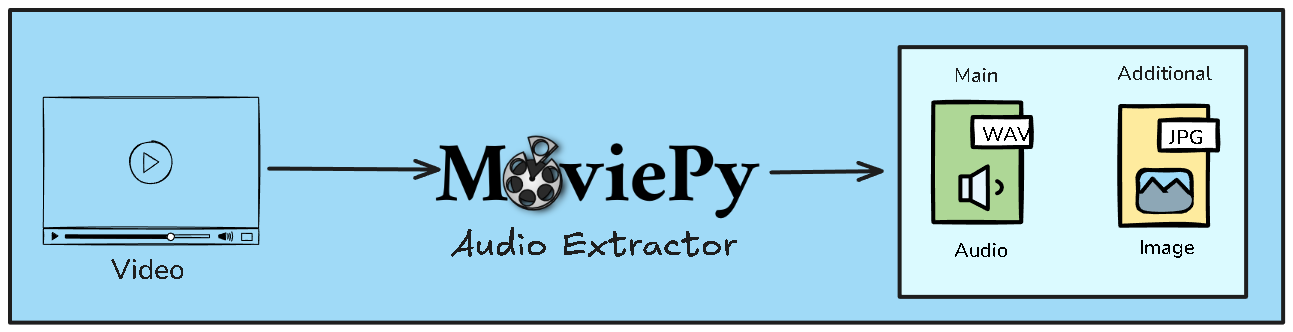
\includegraphics[width=0.8\textwidth]{img/pdz/23-movipy.png}
        \caption{MoviePy Extraction Process.}
        \label{fig:movipy_process}
    \end{figure}
    
    \item \textbf{Audio Transcription}: The extracted audio or raw \texttt{.WAV} files are passed to the \textbf{OpenAI Whisper} ASR engine. Whisper transcribes the speech to text, which is immediately serialized into \textbf{Markdown} format to preserve semantic structure.
    
    \begin{figure}[H]
        \centering
        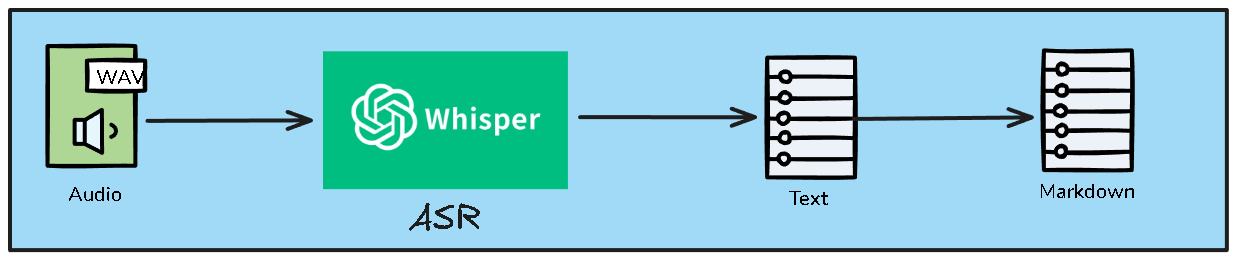
\includegraphics[width=0.8\textwidth]{img/pdz/24-whisper.png}
        \caption{OpenAI Whisper Audio Transcription Process.}
        \label{fig:whisper_process}
    \end{figure}

\end{itemize}

\textbf{Office Document Normalization}

Legacy office formats require conversion before structural analysis. The system utilizes \textbf{LibreOffice} in a headless server environment.
\begin{figure}[H]
    \centering
    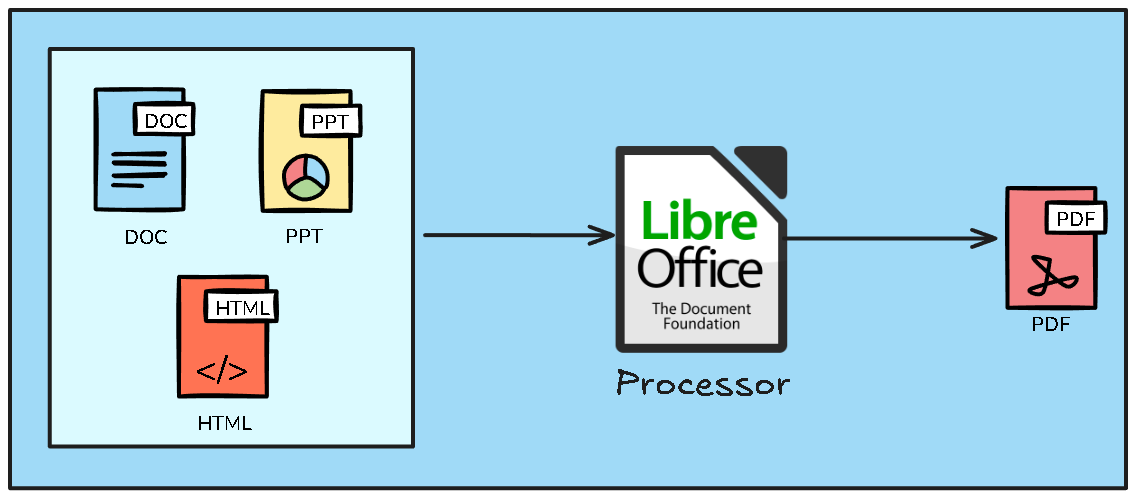
\includegraphics[width=0.8\textwidth]{img/pdz/25-libre.png}
    \caption{LibreOffice Document Conversion Process.}
    \label{fig:libre_process}
\end{figure}

Formats such as Microsoft Word (.DOC), PowerPoint (.PPT), and HTML are normalized into standard \textbf{PDF} documents to freeze layout and fonts.

\textbf{Complex Document Parsing}

For data-dense documents, the pipeline integrates \textbf{Docling} as the central parsing engine:

\begin{figure}[H]
    \centering
    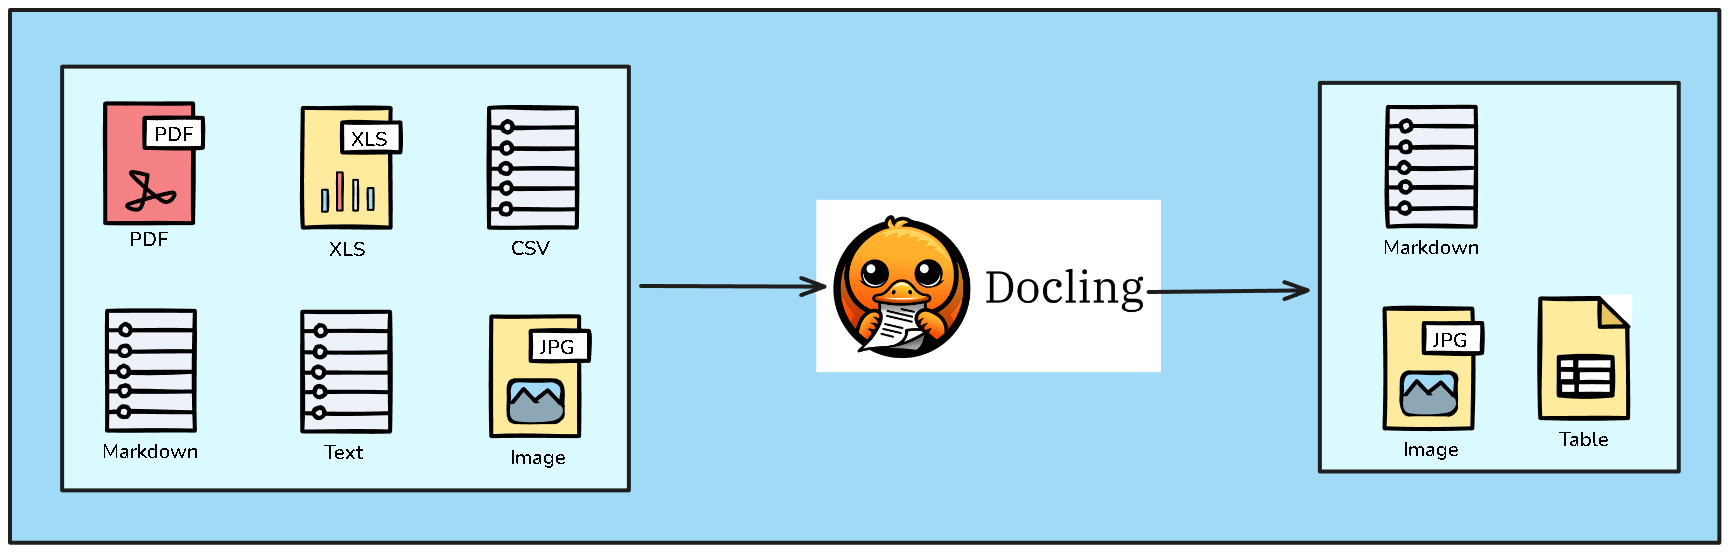
\includegraphics[width=0.8\textwidth]{img/pdz/26-docling.png}
    \caption{Docling Document Parsing Process.}
    \label{fig:docling_process}
\end{figure}

\begin{itemize}
    \item \textbf{Inputs}: Handles PDF, Excel (.XLS), CSV, Markdown, Text, and Images.
    \item \textbf{Outputs}: Docling deconstructs these inputs into three distinct normalized artifacts:
    \begin{enumerate}
        \item \textbf{Structured Markdown}: For semantic text analysis.
        \item \textbf{Table Objects}: For preserving row/column relationships.
        \item \textbf{Isolated Images}: For downstream visual indexing.
    \end{enumerate}
\end{itemize}

\textbf{Output Artifacts}

Every input file results in a unified set of artifacts in the rag ready directory:
\begin{enumerate}
    \item \textbf{PDF}: Used for visual embedding (ColQwen) and user preview.
    \item \textbf{Structured Markdown}: Used for text embedding (BM25/Dense) and LLM context injection.
    \item \textbf{Extracted Metadata}: JSON sidecars containing file provenance, page counts, and processing timestamps.
\end{enumerate}




% \section{Data Preprocessing}
% The preprocessing module transforms raw files into machine-understandable formats. The pipeline splits the workflow into two parallel streams to handle multimodal data:

% \textbf{Text Stream}
% For textual data, the system performs Optical Character Recognition (OCR) or direct text extraction depending on the source file type. The output is standardized into JSON and Markdown formats, stored in the \texttt{output/processing} directory.

% \textbf{Visual Stream}
% A critical component of this pipeline is the handling of visual data within PDFs. The system utilizes \texttt{pdf2image} to render PDF pages into high-resolution images (defaulting to 150 DPI). This rasterization step is essential for the visual retriever (ColQwen), which treats document pages as images to preserve layout and semantic structure that text-only extractors often lose.

% \section{Chunking and Embedding Strategies}
% The system employs a sophisticated "Hybrid + Multimodal" retrieval strategy to maximize recall and precision.

% \textbf{Textual Chunking and Embedding}
% Textual data is segmented into chunks to fit within the context window of the embedding models. The default configuration uses a chunk size of 1000 characters with an overlap of 200 characters. The retrieval mechanism is \textit{Hybrid}, combining two distinct algorithms:
% \begin{enumerate}
%     \item \textbf{Sparse Retrieval (BM25)}: Utilizes keyword matching to capture exact terms and domain-specific jargon.
%     \item \textbf{Dense Retrieval}: Utilizes vector embeddings (stored in FAISS indices) to capture semantic meaning and context. The default embedding model is \texttt{all-MiniLM-L6-v2}.
% \end{enumerate}
% Scores from both retrievers are combined using Min-Max normalization and a weighted sum (default $\alpha=0.5$).

% \textbf{Visual Embedding (ColQwen)}
% Unlike traditional RAG systems that only embed text, this architecture integrates \textbf{ColQwen} (based on ColBERT). This model (specifically \texttt{vidore/colqwen2-v1.0}) generates visual embeddings for document pages, allowing the system to retrieve charts, diagrams, and tables based on visual similarity and visual semantic content. These embeddings are managed via specific quantization settings (e.g., 4-bit or 8-bit) to optimize memory usage.


% \section{Data Preprocessing}

% Following normalization, the data pipeline branches into two specialized processing streams to handle the distinct requirements of textual and visual information. This separation ensures that semantic depth is preserved for text while structural layout is maintained for documents.

% \textbf{Textual Preprocessing Stream}

% The primary input for this stream is the structured \textbf{Markdown} files generated during the normalization phase. The preprocessing logic focuses on preparing this text for semantic vectorization:
% \begin{itemize}
%     \item \textbf{Cleaning}: Removal of artifacts introduced during OCR or file conversion.
%     \item \textbf{Structure Preservation}: The system utilizes the Markdown headers to maintain context, ensuring that section titles remain associated with their respective paragraphs during the splitting process.
% \end{itemize}

% \textbf{Visual Preprocessing Stream}

% For documents rich in diagrams, charts, and complex layouts, the pipeline utilizes the canonical \textbf{PDF} files.
% \begin{itemize}
%     \item \textbf{Rasterization Strategy}: The system implements a "1 Page = 1 Image" conversion strategy. Each PDF page is rendered as a high-resolution JPEG image.
%     \item \textbf{Artifact Management}: These intermediate image files are stored temporarily to facilitate the vision-based embedding process used by ColQwen, ensuring the model "sees" the document exactly as a human would.
% \end{itemize}

\section{Chunking and Embedding Strategies}

The system employs a dual-pathway embedding architecture. This approach allows for the simultaneous retrieval of granular text segments and holistic document pages.

\textbf{Textual Chunking and Embedding}

To process the Markdown inputs, the system utilizes a high-precision splitting strategy designed to maximize retrieval relevance.

\begin{figure}[H]
    \centering
    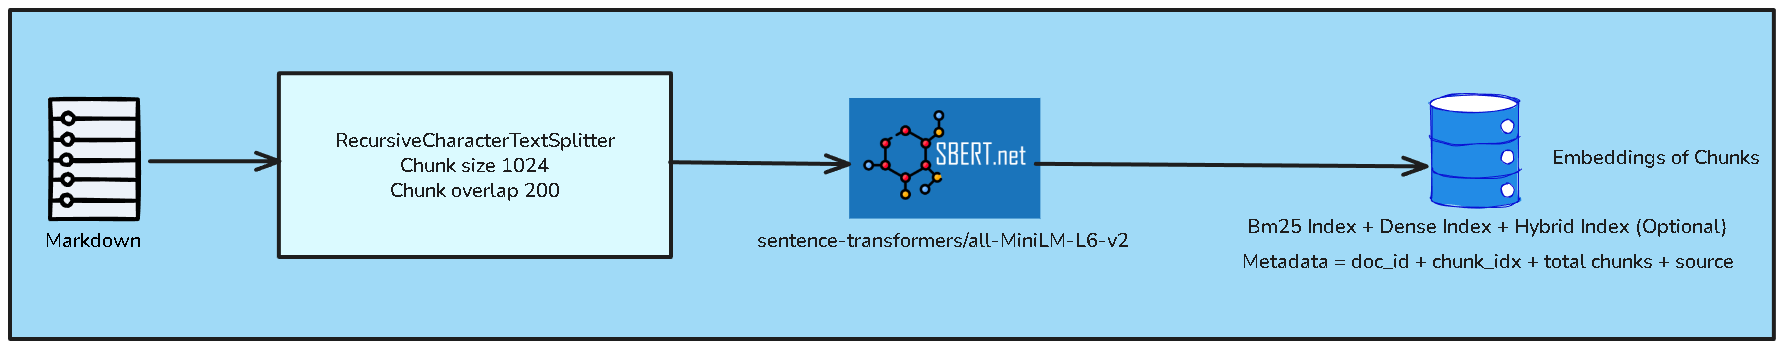
\includegraphics[width=0.8\textwidth]{img/pdz/20-textchunk.png}
    \caption{Textual Chunking and Embedding.}
    \label{fig:textchunk}
\end{figure}

% \textbf{Chunking Logic}

The system employs the \texttt{RecursiveCharacterTextSplitter} with the following specific configuration:
\begin{itemize}
    \item \textbf{Chunk Size}: 1024 characters.
    \item \textbf{Chunk Overlap}: 200 characters.
\end{itemize}
This overlap ensures semantic continuity across chunk boundaries, preventing context loss for sentences that straddle the split point.

\textbf{Text Vectorization (SBERT)}

Processed chunks are mapped to a high-dimensional vector space using the \textbf{Sentence-BERT (SBERT)} framework.
\begin{itemize}
    \item \textbf{Model}: \texttt{sentence-transformers/all-MiniLM-L6-v2}.
    \item \textbf{Output}: A 384-dimensional dense vector representing the semantic meaning of the text chunk.
    \item \textbf{Index Structure}: The embedding is stored alongside a composite metadata object containing:
    \begin{verbatim}
    {
      "doc_id": "unique_document_identifier",
      "chunk_idx": "integer_sequence_number",
      "total_chunks": "total_count_for_document",
      "source": "original_filename"
    }
    \end{verbatim}
\end{itemize}

\textbf{Visual Embedding (ColQwen)}

For documents rich in diagrams, charts, and complex layouts, the pipeline utilizes the canonical \textbf{PDF} files.
The system implements a "1 Page = 1 Image" conversion strategy. Each PDF page is rendered as a high-resolution JPEG image.
These intermediate image files are stored temporarily to facilitate the vision-based embedding process used by ColQwen, ensuring the model "sees" the document exactly as a human would.


The visual pathway processes the page images generated to enable multimodal retrieval.

\begin{figure}[H]
    \centering
    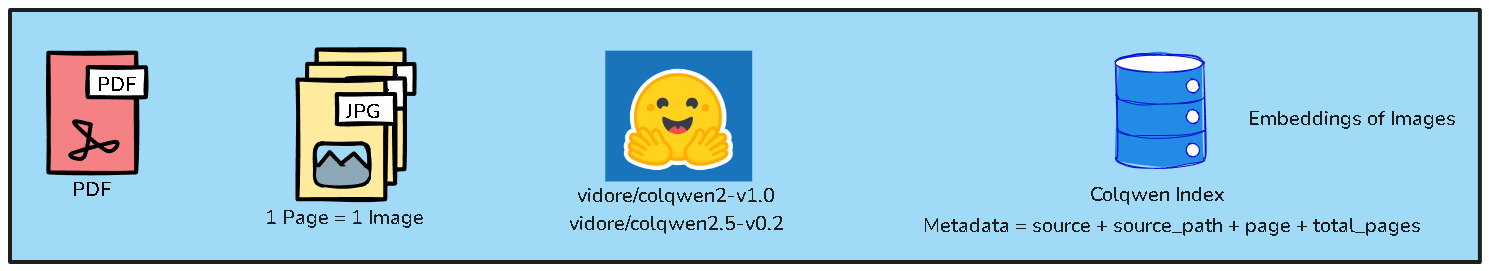
\includegraphics[width=0.8\textwidth]{img/pdz/21-visualemb.png}
    \caption{Visual Embedding (ColQwen).}
    \label{fig:visualemb}
\end{figure}

\textbf{Vision-Language Model}

The system integrates the \textbf{ColQwen} architecture (specifically \texttt{vidore/colqwen2-v1.0} or \texttt{v2.5}). Unlike standard OCR which strips layout, ColQwen encodes the visual semantics of the entire page.

\textbf{Visual Indexing}

\begin{itemize}
    \item \textbf{Embedding Process}: Each rasterized page image is passed through the ColQwen vision encoder to produce visual tokens.
    \item \textbf{Storage}: These embeddings are stored in a specialized ColQwen Index.
    \item \textbf{Metadata Schema}: Visual embeddings are tagged with precise location data:
    \begin{verbatim}
    {
      "source": "original_filename",
      "source_path": "file_system_path_to_pdf",
      "page": "page_number",
      "total_pages": "document_length"
    }
    \end{verbatim}
\end{itemize}

\textbf{Hybrid Retrieval Integration}

The retrieval layer unifies these two streams. The text index supports \textbf{Hybrid Search} (BM25 + Dense), allowing for keyword precision and semantic recall. Optionally, the Text and Visual indices can be queried simultaneously to return both relevant text snippets and their corresponding visual page contexts.


% \section{Database Storage}
% To maintain portability and reduce infrastructure overhead, the system utilizes a \textbf{File-System Based Artifact Store} rather than a traditional relational database. The \texttt{output} directory serves as the database, structured as follows:

% \begin{itemize}
%     \item \textbf{Processed Data}: \texttt{output/processing/} stores the intermediate extraction results in JSON and Markdown.
%     \item \textbf{Text Indices}: \texttt{output/retrieval/} contains the BM25 pickle files (\texttt{.pkl}) and FAISS binary indices (\texttt{.bin}) for text search.
%     \item \textbf{Image Indices}: \texttt{output/image\_retrieval/} stores the ColQwen tensor indices and metadata.
%     \item \textbf{Metadata Store}: JSON files (e.g., \texttt{documents.json}, \texttt{image\_index\_meta.json}) act as the catalog, linking vector IDs back to the original source filenames and page numbers.
% \end{itemize}

% This approach allows the API to perform lightweight status checks by simply reading metadata files (as implemented in the \texttt{/api/status} endpoint), avoiding the need to load heavy models just to check system health.

\newpage